\subsection{Laiko eilučių duomenų dalijimo klasė}
\label{subsec:keystroke_data_splitter}

Klasė \texttt{KeystrokeDataSplitter} iš pradinio CMU CSV failo paruošia \textit{train}, \textit{validation} ir \textit{test} aibes: pasirenka subjektus, normalizuoja požymius ir stratifikuotai padalija duomenis (žr.~\ref{fig:keystroke_data_splitter_class_first} ir \ref{fig:keystroke_data_splitter_class_last} pav.).

\begin{figure}[H]
    \centering
    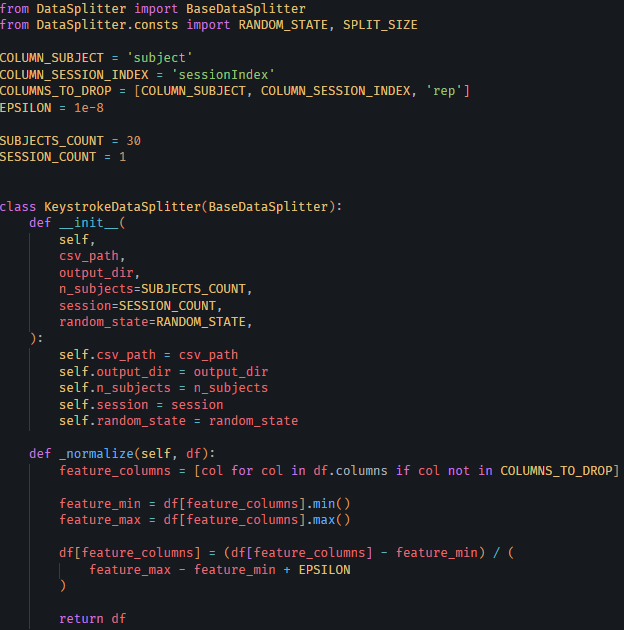
\includegraphics[width=0.85\linewidth]{3Lab/overleaf/images/KeystrokeDataSplitter_Class_1.png}
    \caption{Laiko eilučių duomenų dalijimo klasės kodas I dalis.}
    \label{fig:keystroke_data_splitter_class_first}
\end{figure}

\begin{figure}[H]
    \centering
    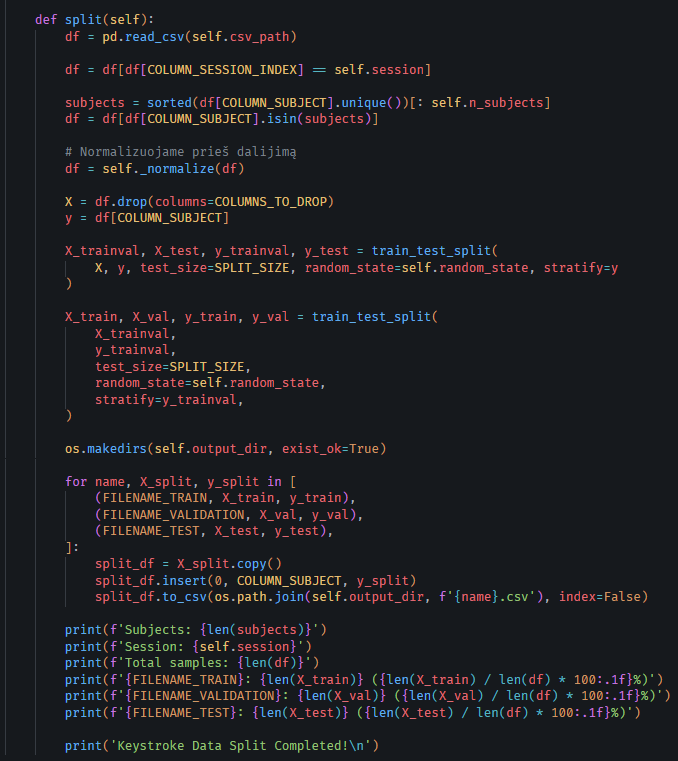
\includegraphics[width=0.85\linewidth]{3Lab/overleaf/images/KeystrokeDataSplitter_Class_2.png}
    \caption{Laiko eilučių duomenų dalijimo klasės kodas II dalis.}
    \label{fig:keystroke_data_splitter_class_last}
\end{figure}

Klasės veikimo žingsniai:
\begin{enumerate}
    \item Iš pradinio CSV nuskaitomos $20\,400$ eilučių; paliekama tik viena sesija (\texttt{sessionIndex}~$=1$).
    \item Iš likusių dalyvių abėcėline tvarka atrenkami pirmieji $30$ subjektai – gauname $30$ klasių klasifikavimo užduotį su $1\,500$ įrašų.
    \item Visi $31$ laikinis požymis normalizuojami min-max metodu į $[0,\,1]$. \texttt{EPSILON}~$=10^{-8}$ apsaugo nuo dalybos iš nulio, jei stulpelio reikšmės sutampa.
    \item Atliekamas dvigubas stratifikuotas dalijimas (\texttt{stratify=y}): pirmas – $80\,\%$ \textit{train+val} ir $20\,\%$ \textit{test}; antras – iš \textit{train+val} aibės dar $80\,\%$ / $20\,\%$ į \textit{train} ir \textit{validation}. Bendras santykis – $64{:}16{:}20$.
    \item Trys gautos aibės įrašomos į atskirus CSV failus, iš kurių vėliau \texttt{KeystrokeDataReader} užkrauna duomenis į \texttt{KeystrokeDataset}.
\end{enumerate}

Klasės kodas parašytas autoriaus. \texttt{sklearn.model\_selection.train\_test\_split} idioma su \texttt{stratify=y} paimta iš \texttt{scikit-learn} oficialios dokumentacijos. Min-max formulę su $\varepsilon$ apsauga padėjo suformuluoti Claude.
